\newpage
\section{Symbolisation}
To gather meaningful information from the entropy profile, and draw any conclusions from the groups of conversations, a symbol model must be established. This section is addressing what was done to establish a working entropy model by figuring out the composition of the symbol set, the model parameters, and what tests/experiments were needed in order to come up with the optimal solutions.

\subsection{Model Goals}
The overall goal for the symbolisation is to isolate a property from both group's resulting entropy profile and increase the margin between them as much as possible, such that the entropy profile shows a visible change in the information when listening to one group vs another. Two obvious properties to isolate are the resulting mean and variance from one group's entropy profile. 
%by aiming to increase the average margin between the two groups mean values and variance values. 
This means constructing a symbol model in such a way that maximises one groups entropy while minimises the others, and maximises consistency in one while minimising in the other. \\

\subsection{Initial Symbol Model}
To produce an informative entropy profile required some knowledge about what the symbol model should look like. Since there was no established methodology to develop an initial proto-symbol model testing this meant composing one from scratch. There were existing, sophisticated techniques for determining potential significant groups in data such as using Machine Learning to cluster data, however for the initial tests this level of sophistication wasn't required. \\

Starting with purely random selections was deemed inefficient. Instead symbol approaches were created that acted as predefined heuristics for constructing new models. This acted as a starting point for the model to be optimised from.  
%Instead pause distributions from the data set were used to see where pauses naturally fell and if they grouped themselves at all as well as symbol approaches that acted as heuristics. 

\subsubsection{Model Constraints}
To help constrain the solution set and find an appropriate solution the models were required to have certain properties.
 
\paragraph{Intragroup Variance} 
The symbol model should maximise capturing meaningful information that is inherent in the specific conversation group. For example, the ranked probability should work well on the ABC conversations data set given its intragroup variance by consistently ranking the symbol model in the same ordering. 

\paragraph{Intergroup Variance}
The symbol model should minimise capturing meaningful information that is inherent to a different group. For example the ranked probability should consistently rank the young group differently from the older group by not capturing the intergroup variance (the most meaningful information for the atypical group would be treated as the same, the model would aim to minimise catering for that groups differences). This can be thought of another way as maximising the margin between the means of the separate entropy profiles. 

\paragraph{Symbol Usage}
Each symbol must have a reliable count that is nonzero and a reliable variance. The entropy can't be calculated for values that have no probability and would cause errors.

\paragraph{Symbol Model Size - Intragroup}
Each symbol should be capturing distinct, atomic, meaningful groups if present. Another constraint would be to make sure there is enough symbols to capture all the potential groups that could carry significant amounts of information. If the groups aren't split enough this means too much information is trying to be conveyed in a single symbol and more than likely will be lost or unstudied. 

\paragraph{Symbol Model Size - Intergroup}
It was important to consider that the symbol model size might be fine for one group but inappropriate for another. An example might occur if too many symbols are used and the data does not exist to utilise them, leaving one or more unused. 
%It can also cause problems if the model is too simple where one symbol might be trying to group too much information and thus might behave unpredictably.

%\subsubsection{Model Strategies}
%Data from the talkbank and abc conversations were pulled out to try and uncover any kind of pattern or insight about how pauses were used by different groups and if they show any similarities between them such as a typical median, mode, mean, or variance value. Something that could be used as a reliable classifier of the data. Ultimately we want to use this to classify atypical physiological or behavioural patterns from typical patterns, but initially we want to use it to classify intra-typical groups as well to see its classification capabilities early on. \\

%A symbol window should have at least 10 occurrences be expected for the selected symbol to use in fast entropy. This presents a lower bound on the window size.
%The threshold for a single window is 10 if we use that as a selected symbol, this doesn't mean we should aim for 10 though. \\

%

%\subsection{Initial Set-up}
%In order to reduce complexity certain areas were left as is or chosen for simplicity first to gain overall insight. Initially pauses were all treated as the same, no distinction was made between joint or inner pause. 

%1ms was used to minimise anomalies being incorrectly picked up and having an effect on the pauses due to the digitisation being too fine grained. 


%\subsection{Data Analysis}
%First passes through model creation looked at the main properties of the audio files that aren't present in the entropy profile. A list of information available with every audio file object included:
%
%\begin{itemize}
%\item Number of Utterances 
%\item Number of Pauses 
%\item Total Binary Pause 
%\item Total Binary Utterance 
%\\
%\end{itemize} 
%
%These were then extended to be:
%
%




%\paragraph{Discussion content}
%What are costs (downsides) of this approach?  What does it mean for the entropy value or the loss of information from pauses to symbols? What are the benefits? \\


%\subsection{Extracting a pause distribution to rank}
%Using a real conversation as an initial example, all the pauses that occurred in the audio file were placed into a distribution. In order to do this, a function was written in calpy that took the already established ndarray of 0's or 1's (where 1's indicate a pause was present) to locate all pauses of at least size 1ms to Xms (whatever X may end up being). The dimension is measured in sizes of 1ms.\\ 

\subsection{Symbolisation Approach 1 (SA1)}
This approach worked by finding a model that maximised entropy by using the histogram for grouping. It starts with a small model size (i.e. starting with a binary model) and a bin width that splits the pauses as evenly as possible by looking at the histogram and seeing where to group pauses. Once a model has been found that maximises entropy for one group this process can be repeated for a ternary model if unsuccessful. 

An example of this would be grouping all the significant meaningful pauses as one symbol for the atypical group, essentially 'erasing' the meaning inherent to that group,  while maximising the meaning for the typical group by symbolising distinct meaningful pauses separately such that it's exclusively catered for. In essence this would have the effect of minimising the entropy values for the atypical group by making it a more predictable system while maximising the entropy values for the second group as there would be less predictability as more information variance is captured separately. 

This can also just be used as a heuristic to show how the information content changes as symbols are added and thresholds are changed. This is the most naive approach but the aim here is simply to maximise entropy with as simple a model as possible for initial testing. It can also provide a good heuristic given that the pauses are already in a ZML like distribution. 
%This approach utilises histograms to see where to group pauses for symbolisation to be as uniform as possible. This approach aims to maximise the margin between groups by maximising one groups entropy. 

%\subsubsection{Cost}
%If entropy is max 



%Look at the histogram and see where you could split the data such that it would be even probability for each symbol.
%Increasing symbol count. This is a heuristic. 

%\subsection{Symbolisation Approach 1.1 (SA1)}
%Extension of SA1. Once symbol model size gets too large it can be hard to see how to maximise entropy without blindly varying symbol thresholds. 
%

%From this a symbol set could be built out of simply splitting up the densest parts of a histogram. 

%it was concluded that any symbol that would cover the first 10ms of pause groups or so would make up the majority of produced symbol set and should thus try to split this proportion evenly. 

%%%%%%%%%%%%%%%%%%%%%%%%%%%%%%%%%%%%%%%%%%%%%%%%%%%%%%%%%%%%%%%%
\subsection{Symbolisation Approach 2 (SA2)}
After more testing was done using symbolisation approach 1, it was found to be effective to use the ranked probability pause comparisons. This was a graph like Figure 5.22 that was used to identify which groups relied on what pauses more often. This was helpful as it showed what pauses showed significant change inter-group and what pauses showed no effect or were similar. This produced a distribution which showed how a clustering could be obtained from the data by examining which sequences of pauses were reliably higher or lower for certain groups. Using this as an identifier meant symbolising those groups. 

\subsubsection{Example}
Figure 5.22 shows two groups, the difference in usage of a particular pause can be identified by the margin between the top of the blue bar group and the yellow dot group. For every individual pause a positive margin can be defined for that pause as the yellow dot group being higher than the blue bar group, zero when they're equal, and negative when the yellow dot group is below the blue bar group. 

\begin{figure}[htbp]
\begin{center}
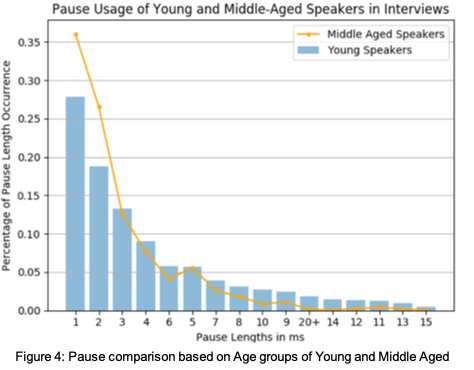
\includegraphics[scale=1.4]{src/main-matter/methodology/symbolisation/pause-difference-intergroup}
\caption{Ranked probability plot showing how pauses can be ranked. This provides insight into where meaningful groups exist in both data sets and how to best symbolise these pause groups.}
\label{default}
\end{center}
\end{figure}


\paragraph{Example Symbolisation 1}
A symbol model for this data could collect all the margins that are positive as one symbol, all margins that are 0 as another, and all margins that are negative as a final symbol. This would produce a 3 symbol model. This could be extended with parameters that define at what point a margin would be positive, negative, neutral (i.e. allow for a 5\% variance for neutral values). 


\paragraph{Example Symbolisation 2}
Another approach could be to extend approach 1 and also focus on the locality of the pauses such as grouping the margins that are next to each other and also of similar margin type (positive, negative, neutral) as a single symbol. This would produce as symbolisation as shown in Figure 5.23. The author was at the discretion to choose where the neutral group existed, thus 


\begin{figure}[htbp]
\begin{center}
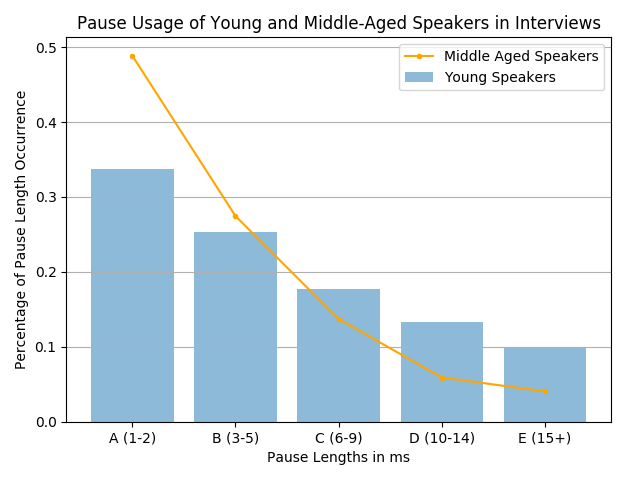
\includegraphics[scale=0.7]{src/main-matter/methodology/symbolisation/dual_binary_pause_bar_chart}
\caption{Ranked symbol usage shows an example symbol model created using SA2 and its symbol ranking after being tested}
\label{default}
\end{center}
\end{figure}

\subsubsection{Improvement}
%From here a symbol model was built. 
With this a symbol model can then be optimised gradually through iterations. The iterations consist of running tests and and comparing to another group, measuring effectiveness, then going back to the pause distribution and adjusting pauses to create different symbol sets to see how the shift will impact on subsequent entropy profiles (repeat as necessary). This approach can be thought of as being similar to SA1, except the aim here is just to try and increase the margin without necessarily maximising the entropy for a single group.



\subsection{Symbolisation Approach 3 (SA3)}
This approach aims to produce a ranked probability model that is invariant to intragroup change, but variant to intergroup change, by reordering the ranked probability model should an audio file be symbolised that disrupts the expected symbol ranking. From the constraints the model needs to be have a wide enough margin of error present between symbols that it can handle small intragroup variance between speakers but not too large that it also captures the other groups incorrectly. Requiring the margin of error being optimised can make finding an appropriate solution difficult. This could be implemented through requiring a portion of the total pause occurrence be present between symbols, for example if 2,000 pauses occurred then aiming for a 5\% gap of 100 pauses between symbol A and symbol B would help with stability. The actual percentage would be worked out through iterative testing. This template model, $M$, would take in the number of symbols present in the model, $n$, and the margin between, $m$. $M(n, m) = \sum_{i=0}^n (x - i*m)$ where $x$ is solved for as an unknown when $ M = 100$. In the instance where $n = 3, m = 5\%$, this would be $x = 38.333$ and symbol$ A = x - 0(5)$, symbol $B = x - 1(5)$, symbol $C = x - 2(5)$. This would require knowing the optimal margin as well between symbols which would require measurement to find. This approach would then need to fit with the actual data available by finding the symbol model that most closely matches the calculated percentages for each symbol.

Symbol models should aim to not use too few or too many symbols. Otherwise a minority of symbols carry the majority of meaning. only a few symbol can be used as one symbol will record a majority of the pause readings leaving little for the other symbols (and if that happens it will be very hard to detect noticeable change as it would require a large amount of change to change the ranked probability, i.e. hard to capture the intergroup variance). This is more of a heuristic than anything and as such it is flexible as long as it is the model is reliable and each symbol is not 0 or too large in use. Symbols should either break apart if too large or join if too small. 

Another strategy is to find the difference in usage between symbol sets and maximise the difference each symbol while minimising the number of symbols (such that each symbol will capture a 'run' of difference).



%\subsection{Symbolisation Approach 4 (SA4)}
%As mentioned in the Intergroup Variance constraint above, the symbol model should aim to increase the entropy of one model significantly while decreasing the mean entropy of the other. This will make classifications between the two groups more prominent when change does occur. 


\subsection{Symbolisation Approaches}
For this thesis only SA1 and SA2 were used in the experiments. SA3 was developed as a potential alternatives to be considered alongside SA1 and SA2 should they not work.